\chapter{Letture}

Questo capitolo contiene dei mini-riassunti delle Letture
obbligatorie per l'esame. Poiché è possibile e consigliato consultare
i documenti durante l'esame, questi riassunti hanno la funzione di 
aiutare a ricordare i concetti principali per facilitare la navigazione 
e la consultazione.

\begin{itemize}
    \item [$\Rightarrow$] Vannevar Bush, \href{https://informatica.i-learn.unito.it/pluginfile.php/368484/mod_resource/content/7/Bush%20%281945%29.pdf}{Come potremmo pensare}, 1945;
    \item [$\Rightarrow$] Susan Barnes, \href{https://informatica.i-learn.unito.it/pluginfile.php/368474/mod_resource/content/2/Barnes%2C%20S.B.%20--%20Douglas%20Carl%20Engelbart-%20developing%20the%20underlying%20concepts%20for%20contemporary%20computing.pdf}{Douglas Carl Engelbart: Developing the Underlying Concepts for Contemporary Computing}, 1997;
    \item [$\Rightarrow$] J. C. R. Licklider, \href{https://informatica.i-learn.unito.it/pluginfile.php/368452/mod_resource/content/2/Licklider%20-%20Man-Computer%20Symbiosis.pdf}{Man-computer symbiosis}, 1960;
    \item [$\Rightarrow$] Lev Manovich, \href{https://informatica.i-learn.unito.it/pluginfile.php/368438/mod_resource/content/1/Lev%20Manovich-Software_Takes_Command-Ch1.pdf}{Alan Kay's Universal Media Machine}, 2013.
\end{itemize}

\nt{Inoltre per "Man-computers symbiosis" è presente questa traduzione in italiano: \href{https://informatica.i-learn.unito.it/mod/resource/view.php?id=238398}{Simbiosi uomo-computer}.
}
\section{Come potremmo pensare}

\paragraph{Introduzione, sezione 1 e sezione 2:} l'articolo si apre con una riflessione sulla seconda guerra mondiale (infatti l'articolo è del '45)
in cui vari scienziati (in particolare fisici) hanno contribuito allo sforzo bellico invece che alla ricerca.
Subito dopo si passa a parlare del fenomeno dell'accumulo di conoscenza (\fancyglitter{Information Overload}) e
di come il problema non fosse l'eccesso di informazione, ma la mancanza di strumenti per gestirla\footnote{
    Come esempio vengono viste le leggi della genetica di Mendel, passate inosservate per una generazione.
}.
Successivamente si parla della question costi-benefici relativa all'utilizzo di determinate tecnologie\footnote{
    Nè la macchina per i calcoli di Leibniz, nè la macchina analitica di Babbage sono state realizzate.
}.

\paragraph{Sezione 3:} è presente una descrizione di un sistema per convertire la voce in testo, che permetterebbe
di velocizzare la scrittura di documenti e lascerebbe più tempo per la riflessione. Si parla di \fancyglitter{meccanizzazione
di processi ripetitivi}\footnote{Collegamento a Licklider, "Man-computer symbiosis"} e di come, in futuro,
si potrebbero avere macchine in grado di fare ragionamenti complessi a velocità molto elevate\footnote{
    Tali macchine saranno controllate mediante schede o pellicole (i microfilm adorati da Bush).
}.

\paragraph{Sezione 4} si parla di come il matematico non sia una persona che fa calcoli, ma una persona che risolve problemi
logici complessi (ad alto livello) e che per questo dovrebbe delegare i calcoli, anche di complessità elevata, a macchine. 
In futuro potranno esistere macchine sufficientemente meticolose da poter soddisfare
anche i matematici più esigenti.

\paragraph{Sezione 5:} si parla di macchine in grado di fare ragionamenti logici prendendo in input delle premesse e restituendo
delle conclusioni. Per fare ciò nascerà un nuovo simbolismo, probabilmente posizionale. Inoltre non ci si limiterà a manipolare la logica,
ma anche le \fancyglitter{idee}. Dopo di ché, Bush, ritorna al problema della \fancyglitter{selezione} con l'esempio di 
un impiegato che deve trovare tutti gli impiegati che vivono a Trenton e conoscono lo spagnolo (lo fa tramite una macchina selezionatrice\footnote{
    Ricorda una SELECT in SQL.
}).
Però questa è una selezione semplice. Un altro esempio è quello di una centralina telefonica che deve connettersi a un'altra 
centralina, quindi senza ispezionare tutte le linee, ma solo quella che interessa. Termina
la sezione con ulteriori esempi e cita le \fancyglitter{biblioteche}.

\paragraph{Sezione 6 e sezione 7:} finalmente si parla del problema dell'\fancyglitter{indicizzazione}. Il problema è che la mente umana 
non funziona per indicizzazione, ma per \fancyglitter{associazione}, facendo continui collegamenti tra idee\footnote{Ipertesti.}.
Difficilmente ciò può essere meccanizzato perfettamente al 100\%, ma si può, in parte, emulare. Questa 
è l'idea alla base del \fancyglitter{Memex}\footnote{Anche qua Bush si lascia trascinare dall'amore per i microfilm.}.
Bush parla di come sia importante il processo di collegare due elementi insieme. Nella 
settima sezione si fa un esempio del Memex che si vedrà nel famoso filmato.

\paragraph{Sezione 8:} Bush parla di nuovi tipi di enciclopedie fruibili da tutti e personalizzate sulla base 
delle esigenze dell'utente. Inoltre viene introdotta la professione di \fancyglitter{apripista} (o trail blazers\footnote{Honkai Star Rail refernce.}):
persone che si occupano di creare nuovi collegamenti tra idee. Le ultime pagine sono dedicate a delle riflessioni
di natura più filosofica che consiglio di leggere.

\section{Douglas Carl Engelbart: Developing the Underlying Concepts for Contemporary Computing}

\paragraph{Introduzione:} si parla dei progressi della tecnologia dovuti alle idee di Engelbart\footnote{
    Mouse, GUI, etc.
}. Queste idee diventarono le fondamenta della moderna informatica.

\paragraph{Influenze della formazione:} viene descritta la formazione di Engelbart e come questa abbia influenzato il suo lavoro.
In particolare si parla di come "\fancyglitter{As We May Think}" di Bush, letto dopo la seconda guerra mondiale, lo abbia 
spinto a perseguire una carriera nello sviluppo di \fancyglitter{strumenti per la conoscenza}. Engelbart cercava
uno scopo nella vita che non fosse solo il guadagno personale, ma che potesse aiutare l'umanità.

\paragraph{Il concetto iniziale di Augmentation:} si inizia con il tempo trascorso da Engelbart alla Stanford Research Institute (SRI), dal 1957.
Nel 1962 viene pubblicato "Augmenting Human Intellect: A Conceptual Framework" in cui si parla di come la tecnologia
possa essere usata per aumentare l'intelletto umano. L'anno succesivo espone l'idea di aumentare l'intelletto umano
partendo dai processi di informazione che possono essere:

\begin{itemize}
    \item [$\Rightarrow$] \fancyglitter{Consci:} processi che l'individuo è consapevole di fare. Per 
    esempio, riconoscere pattern, visualizzare, astrarre, dedurre, etc.;
    \item [$\Rightarrow$] \fancyglitter{Inconsci:} processi che l'individuo non è consapevole di fare. Per esempio,
    l'informazione autogenerata.
\end{itemize}

\paragraph{L'aumento dell'intelletto umano si divide in 4 classi:}

\begin{itemize}
    \item [$\Rightarrow$] \fancyglitter{Artefatti};
    \item [$\Rightarrow$] \fancyglitter{Linguaggio};
    \item [$\Rightarrow$] \fancyglitter{Metodologia};
    \item [$\Rightarrow$] \fancyglitter{Addestramento}.
\end{itemize}

\nt{Queste cose sono viste in dettaglio nel capitolo \ref{augmentation}.}

\begin{figure}[h]
    \centering
    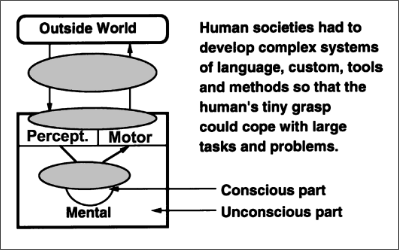
\includegraphics[scale=0.5]{images/Mondo.png}
    \caption{Visione del mondo.}
    \label{fig:Engelbart}
\end{figure}

\subsubsection{}

Per Engelbart l'addestramento è necessario per poter utilizzare i nuovi strumenti. Es. 
un aborigeno non addestrato non riuscirebbe a utilizzare una macchina, ma con il giusto addestramento composto da \fancyglitter{piccoli step}
potrebbe farlo. Infatti si impara meglio con piccoli step che con un'unica grande lezione.

\paragraph{Manipolazione simbolica:} parla dell'attività chiamata "pensiero" e di come gli esseri
umani riescano a effettuare astrazioni e \fancyglitter{manipolazione concettuale} (primo stadio di sviluppo).
Successivamente passano alla \fancyglitter{manipolazione simbolica} (secondo stadio di sviluppo) in cui si manipolano
simboli che rappresentano concetti. Il terzo stadio di sviluppo consiste nella manipolazione simbolica mediante \fancyglitter{grafici}\footnote{Questo 
è derivato dal linguaggio che si utilizza.
}. Il quarto stadio è l'unione del terzo con la componente linguistica.

\paragraph{Computazione interattiva:} Si parla della maggiore simbiosi tra uomo e macchina. Viene anche portato in evidenza il
"\fancyglitter{Bootstrap}", ossia un metodo per analizzare e migliorare il proprio lavoro in team.

\begin{figure}[h]
    \centering
    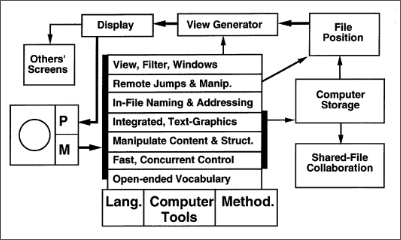
\includegraphics[scale=0.5]{images/Au.png}
    \caption{Aumentazione.}
\end{figure}

\paragraph{Supporto da ARPA:} Viene descritto il supporto che Engelbart ha ricevuto da Licklider (grazie ad ARPA) e, successivamente,
da Taylor (NASA).

\paragraph{THe Augmentation Research Center:} In questo capitolo si parla della creazione del \fancyglitter{The Augmentation Research Center} (ARC) e 
della tecnologia che è stata sviluppata al suo interno, ossia il \fancyglitter{NLS} (o \fancyglitter{oN-Line System}).
NLS è un sistema che permette di fare molte cose, tra cui la condivisione di documenti, la creazione di documenti, mail, etc.
Inoltre si parla di altri dispositivi come un oggetto che si utilizzava con una mano e aveva 5 tasti (per esempio I - insert, D - delete, etc.), ma ebbe poco successo per via dei
possibili crampi ai muscoli. Oltre a ciò veniva utilizzato un mouse analogico.

\paragraph{The Mother of All Demos (Demonstration):} Engelbart spese la maggior parte dei suoi fondi per la DEMO 
del '68, doveva essere un successo e così fu. Il capitolo si concentra su una descrizione della presentazione della DEMO.

\paragraph{Su ARPANET:} Viene descritto ARPANET (il cui secondo nodo fu ARC) e come sia stato il precursore di Internet, anche grazie a NLS.

\paragraph{Conclusione:} Si parla del declino del team di Engelbart al SRI e di come i suoi membri 
si trasferirono allo Xerox PARC. Si chiude con una considerazione riguardo al fatto che Engelbart non sia
famoso o ricco sebbene il suo lavoro abbia avuto un impatto enorme sul Web e sul concetto di personal computer.

\section{Man-computer symbiosis}

\paragraph{Introduzione:} Licklider inizia descrivendo la collaborazione tra uomo e macchina e la sua speranza che 
in futuro si possa avere una simbiosi tra i due. 

\paragraph{Scopo della simbiosi uomo-macchina:} Ci sono due scopi principali:

\begin{itemize}
    \item [$\Rightarrow$] Portare le macchine nella parte formulativa del pensiero;
    \item [$\Rightarrow$] Pensare in tempo reale.
\end{itemize}

\paragraph{Necessità della partecipazione del computer alla formulazione e 
pensare in tempo reale:} Viene descritto come l'85\% del tempo di un uomo sia speso nel 
mettersi in condizione di poter pensare, ma solo il 15\% nel pensare effettivamente.
Inoltre si parla di come il linguaggio umano sia ridondante rispetto a quello delle macchine.

\paragraph{Funzioni separabili di uomini e computer in anticipazione dell'associazione
simbiotica:} 

\begin{itemize}
    \item [$\Rightarrow$] Gli uomini si dovrebbero occupare degli obiettivi e delle ipotesi.
    Sono loro a porre i problemi e pensare a procedure e modelli. Oltre a gestire situazioni impreviste;
    \item [$\Rightarrow$] I computer si dovrebbero occupare di convertire le ipotesi in modelli 
    testabili e di testarli. Inoltre dovrebbero gestire i dettagli e le procedure. Oltre a ciò 
    i computers serviranno a fare inferenza statistica, teoria delle decisioni, teoria dei giochi, etc.
\end{itemize}

\paragraph{Prerequisiti per la realizzazione della simbiosi uomo-computer:}

\begin{itemize}
    \item [$\Rightarrow$] Differenza di velocità tra uomo e macchina: la velocità del computer 
    deve essere bilanciata con quella dell'uomo;
    \item [$\Rightarrow$] Requisiti di memoria hardware: una parte deve essere indelebile, mentre
    un'altra deve essere modificabile;
    \item [$\Rightarrow$] Requisiti di organizzazione della memoria: devono esserci specifici meccanismi
    che garantiscono l'efficienza nel recuperare informazioni;
    \item [$\Rightarrow$] Il problema del linguaggio: il computer deve essere in grado di comprendere
    un linguaggio. Per esempio il FORTRAN o l'ALGOL;
    \item [$\Rightarrow$] Equipaggiamento per l'input e l'output:
    \begin{itemize}
        \item Display e controlli;
        \item Wall display;
        \item Produzione e riconoscimento vocale.
    \end{itemize}
\end{itemize}

\section{Alan Kay's Universal Media Machine}

Si tratta del primo capitolo di un libro che parla dei principali
contributi di alcuni personaggi chiave per lo sviluppo dell'informatica.
Questo capitolo si concentra su Alan Kay.

